% Define all input paths
\makeatletter
\def\input@path{%
  {./styles/}%
  {./content/appendices/}%
  {./content/sections/}%
  {./content/sections/section_1/}%
  {./content/sections/section_2/}%
  {./content/sections/section_4/}%
  {./content/sections/section_5/}%
  {./content/sections/section_6/}%
  {./content/sections/section_7/}%
}
\makeatother

% Define commands for importing from specific sections
\newcommand{\inputSectionOne}[1]{\input{./content/sections/section_1/#1}}
\newcommand{\inputSectionTwo}[1]{\input{./content/sections/section_2/#1}}
\newcommand{\inputSectionThree}[1]{\input{./content/sections/section_3/#1}}
\newcommand{\inputSectionFour}[1]{\input{./content/sections/section_4/#1}}
\newcommand{\inputSectionFive}[1]{\input{./content/sections/section_5/#1}}
\newcommand{\inputSectionSix}[1]{\input{./content/sections/section_6/#1}}
\newcommand{\inputSectionSeven}[1]{\input{./content/sections/section_7/#1}}
\newcommand{\inputAppendix}[1]{\input{./content/appendices/#1}}


\documentclass[11pt]{article}
\usepackage[margin=1in]{geometry}
\usepackage{hyperref}
\usepackage{xcolor}
\usepackage{listings}
\usepackage{tcolorbox}
\usepackage{enumitem}
\usepackage{fancyvrb}
\usepackage{tikz}
\usetikzlibrary{positioning} 
\usepackage{pgfplots}
\usepackage{booktabs}
\usepackage{array}
\usepackage{endnotes}
\usepackage{hyperendnotes}

\title{\textbf{hyperendnotes.sty}\\[0.5em]\Large Comprehensive Documentation and Technical Reference}
\author{Package Technical Documentation}
\date{\today}

\newcommand{\code}[1]{\texttt{#1}}
\newcommand{\pkg}[1]{\textsf{#1}}
\newcommand{\cmd}[1]{\texttt{\textbackslash#1}}
\newcommand{\cmdwithargs}[2]{\texttt{\textbackslash#1\{#2\}}}
\newcommand{\file}[1]{\texttt{#1}}

\lstset{
  basicstyle=\ttfamily\small,
  breaklines=true,
  breakatwhitespace=true,
  commentstyle=\color{gray},
  frame=single,
  keepspaces=true,
  keywordstyle=\color{blue},
  language=[LaTeX]TeX,
  showspaces=false,
  showstringspaces=false,
  stringstyle=\color{purple},
  tabsize=2,
  morekeywords={endnote,endnotemark,endnotetext,theendnotes,enotelinkstrue,enotelinksfalse},
  escapechar=|
}

\DefineVerbatimEnvironment{codeblock}{Verbatim}{fontsize=\small, frame=single, framesep=2mm, numbers=left, xleftmargin=5mm}

\tikzset{
  process/.style={rectangle, rounded corners, minimum width=3cm, minimum height=1cm, text centered, draw=blue},
  arrow/.style={thick,->,>=stealth},
  annotation/.style={text width=4cm, font=\footnotesize}
}

\begin{document}

\maketitle

\tableofcontents

\newpage
\section{Introduction}

The \pkg{hyperendnotes} package enhances the standard \pkg{endnotes} package by adding comprehensive hyperlink functionality. It creates an interactive document experience with bidirectional navigation between endnote references in the text and the actual endnotes listed at the document's end. This documentation provides a detailed technical explanation of the package's functionality, implementation details, and usage examples.

\subsection{Purpose}

The main purposes of the \pkg{hyperendnotes} package are:

\begin{itemize}
  \item To create hyperlinks from endnote marks in the text to their corresponding endnotes
  \item To create back-references from each endnote to its position in the text
  \item To preserve hyperlink functionality within endnote content
  \item To provide a mechanism to toggle this hyperlink functionality
  \item To maintain compatibility with the core functionality of the \pkg{endnotes} package
\end{itemize}

\subsection{Package Dependencies}

The \pkg{hyperendnotes} package requires:

\begin{itemize}
  \item \pkg{endnotes} -- Provides the base endnote functionality
  \item \pkg{hyperref} -- Provides hyperlink capabilities
\end{itemize}

Both packages must be loaded before \pkg{hyperendnotes}.

\section{Package Implementation Analysis}

This section provides a detailed analysis of the \pkg{hyperendnotes} implementation, explaining each component's purpose and functionality.

\subsection{Core Package Variables}

\begin{tcolorbox}[colback=gray!5, colframe=gray!75, title=Core Variables]
\begin{lstlisting}
\makeatletter
\newif\ifenotelinks
\newcounter{Hendnote}
\let\savedhref\href
\let\savedurl\url
\end{lstlisting}
\end{tcolorbox}

The package defines:
\begin{itemize}
  \item \cmd{ifenotelinks} -- A boolean toggle for enabling/disabling hyperlinks
  \item \cmd{Hendnote} -- A counter for hyperlink targets
  \item \cmd{savedhref} and \cmd{savedurl} -- Saved versions of the hyperref commands to use within endnotes
\end{itemize}

\subsection{Endnote Command Redefinitions}

The package redefines several commands from the \pkg{endnotes} package to add hyperlink functionality. Let's examine each redefined command:

\subsubsection{\cmd{endnotemark} Command}

\begin{tcolorbox}[colback=gray!5, colframe=gray!75, title=endnotemark Redefinition]
\begin{lstlisting}
\def\endnotemark{%
\@ifnextchar[\@xendnotemark{%
\stepcounter{endnote}%
\protected@xdef\@theenmark{\theendnote}%
\protected@xdef\@theenvalue{\number\c@endnote}%
\@endnotemark
}%
}%
\end{lstlisting}
\end{tcolorbox}

This redefines the \cmd{endnotemark} command to:
\begin{itemize}
  \item Check if an optional argument is provided
  \item Increment the endnote counter if no argument is provided
  \item Store the formatted endnote number in \cmd{@theenmark}
  \item Store the raw endnote counter value in \cmd{@theenvalue} (needed for hyperlinks)
  \item Call the internal \cmd{@endnotemark} command
\end{itemize}

\subsubsection{\cmd{@xendnotemark} Command}

\begin{tcolorbox}[colback=gray!5, colframe=gray!75, title=@xendnotemark Redefinition]
\begin{lstlisting}
\def\@xendnotemark[#1]{%
\begingroup\c@endnote#1\relax
\unrestored@protected@xdef\@theenmark{\theendnote}%
\unrestored@protected@xdef\@theenvalue{\number\c@endnote}%
\endgroup
\@endnotemark
}%
\end{lstlisting}
\end{tcolorbox}

This redefined command handles the case when an optional argument (specific endnote number) is provided:
\begin{itemize}
  \item Sets the endnote counter to the specified value
  \item Stores the formatted endnote number and raw counter value
  \item Calls the internal \cmd{@endnotemark} command
\end{itemize}

\subsubsection{\cmd{endnotetext} Command}

\begin{tcolorbox}[colback=gray!5, colframe=gray!75, title=endnotetext Redefinition]
\begin{lstlisting}
\def\endnotetext{%
\@ifnextchar[\@xendnotenext{%
\protected@xdef\@theenmark{\theendnote}%
\protected@xdef\@theenvalue{\number\c@endnote}%
\@endnotetext
}%
}%

\def\@xendnotenext[#1]{%
\begingroup
\c@endnote=#1\relax
\unrestored@protected@xdef\@theenmark{\theendnote}%
\unrestored@protected@xdef\@theenvalue{\number\c@endnote}%
\endgroup
\@endnotetext
}%
\end{lstlisting}
\end{tcolorbox}

These redefinitions handle adding endnote text without placing a mark, with similar functionality as above but calling \cmd{@endnotetext} instead.

\subsubsection{\cmd{endnote} Command}

\begin{tcolorbox}[colback=gray!5, colframe=gray!75, title=endnote Redefinition]
\begin{lstlisting}
\def\endnote{%
\@ifnextchar[\@xendnote{%
\stepcounter{endnote}%
\protected@xdef\@theenmark{\theendnote}%
\protected@xdef\@theenvalue{\number\c@endnote}%
\@endnotemark\@endnotetext
}%
}%

\def\@xendnote[#1]{%
\begingroup
\c@endnote=#1\relax
\unrestored@protected@xdef\@theenmark{\theendnote}%
\unrestored@protected@xdef\@theenvalue{\number\c@endnote}%
\show\@theenvalue
\endgroup
\@endnotemark\@endnotetext
}%
\end{lstlisting}
\end{tcolorbox}

The \cmd{endnote} command combines the functionality of \cmd{endnotemark} and \cmd{endnotetext}, placing both a mark in the text and adding the corresponding note.

\subsubsection{\cmd{@endnotemark} Command}

\begin{tcolorbox}[colback=gray!5, colframe=gray!75, title=@endnotemark Redefinition]
\begin{lstlisting}
\def\@endnotemark{%
\leavevmode
\ifhmode
\edef\@x@sf{\the\spacefactor}\nobreak
\fi
\ifenotelinks
\expandafter\@firstofone
\else
\expandafter\@gobble
\fi
{%
\Hy@raisedlink{%
\hyper@@anchor{Hendnotepage.\@theenvalue}{\empty}%
}%
}%
\hyper@linkstart{link}{Hendnote.\@theenvalue}%
\makeenmark
\hyper@linkend
\ifhmode
\spacefactor\@x@sf
\fi
\relax
}%
\end{lstlisting}
\end{tcolorbox}

This is a key redefinition that adds hyperlink functionality to the endnote mark:
\begin{itemize}
  \item Preserves the space factor (spacing between characters)
  \item Creates a hyperlink anchor at the endnote reference position if links are enabled
  \item Creates a hyperlink from the endnote mark to the actual endnote
  \item Restores spacing properties
\end{itemize}

\subsubsection{\cmd{@endnotetext} Command}

\begin{tcolorbox}[colback=gray!5, colframe=gray!75, title=@endnotetext Redefinition]
\begin{lstlisting}
\long\def\@endnotetext#1{%
\if@enotesopen
\else
\@openenotes
\fi
\immediate\write\@enotes{%
\@doanenote{\@theenmark}{\@theenvalue}%
}%
\begingroup
\def\next{#1}%
\newlinechar='40
\immediate\write\@enotes{\meaning\next}%
\endgroup
\immediate\write\@enotes{%
\@endanenote
}%
}%
\end{lstlisting}
\end{tcolorbox}

This redefinition writes the endnote content to the auxiliary file, but now includes the raw endnote number (\cmd{@theenvalue}) for hyperlink creation.

\subsection{Endnote Rendering Redefinitions}

\subsubsection{\cmd{theendnotes} Command}

\begin{tcolorbox}[colback=gray!5, colframe=gray!75, title=theendnotes Redefinition]
\begin{lstlisting}
\def\theendnotes{%
\immediate\closeout\@enotes
\global\@enotesopenfalse
\begingroup
\makeatletter
\edef\@tempa{`\string>}%
\ifnum\catcode\@tempa=12
\let\@ResetGT\relax
\else
\edef\@ResetGT{\noexpand\catcode\@tempa=\the\catcode\@tempa}%
\@makeother\>%
\fi
\def\@doanenote##1##2##3>{%
\def\@theenmark{##1}%
\def\@theenvalue{##2}%
\par
\smallskip %<-small vertical gap between endnotes
\begingroup
\def\href{\expandafter\savedhref}%
\def\url{\expandafter\savedurl}%
\@ResetGT
\edef\@currentlabel{\csname p@endnote\endcsname\@theenmark}%
\enoteformat
}%
\def\@endanenote{%
\par\endgroup
}%
% Redefine, how numbers are formatted in the endnotes-section:
\renewcommand*\@makeenmark{%
\hbox{\normalfont\@theenmark~}%
}%
% header of endnotes-section
\enoteheading
% font-size of endnotes
\enotesize
\input{\jobname.ent}%
\endgroup
}%
\end{lstlisting}
\end{tcolorbox}

This redefinition:
\begin{itemize}
  \item Closes the endnotes auxiliary file
  \item Handles special character category codes to ensure proper parsing
  \item Redefines the \cmd{@doanenote} command to process each endnote with hyperlink information
  \item Restores \cmd{href} and \cmd{url} functionality within endnotes
  \item Sets formatting for endnote marks in the endnotes section
  \item Inputs the generated endnotes file to display all endnotes
\end{itemize}

\subsubsection{\cmd{enoteformat} Command}

\begin{tcolorbox}[colback=gray!5, colframe=gray!75, title=enoteformat Redefinition]
\begin{lstlisting}
\def\enoteformat{%
\rightskip\z@
\leftskip1.8em
\parindent\z@
\leavevmode\llap{%
\setcounter{Hendnote}{\@theenvalue}%
\addtocounter{Hendnote}{-1}%
\refstepcounter{Hendnote}%
\ifenotelinks
\expandafter\@secondoftwo
\else
\expandafter\@firstoftwo
\fi
{\@firstofone}%
{\hyperlink{Hendnotepage.\@theenvalue}}%
{\makeenmark}%
}%
}%
\end{lstlisting}
\end{tcolorbox}

This command defines how each endnote is formatted in the endnotes section:
\begin{itemize}
  \item Sets paragraph formatting properties
  \item Handles the endnote number counter for hyperlinks
  \item Creates a back-reference hyperlink from the endnote to its position in the text
  \item Formats the endnote mark according to the defined style
\end{itemize}

\subsection{Package Toggle Commands}

\begin{tcolorbox}[colback=gray!5, colframe=gray!75, title=Toggle Commands]
\begin{lstlisting}
\makeatother
% Toggle switch in order to turn on/off back-links in the
% endnote-section:
\enotelinkstrue
%\enotelinksfalse
\end{lstlisting}
\end{tcolorbox}

The package provides two commands to enable or disable hyperlinks:
\begin{itemize}
  \item \cmd{enotelinkstrue} -- Enable hyperlinks (default)
  \item \cmd{enotelinksfalse} -- Disable hyperlinks
\end{itemize}

\section{Usage Guide}

\subsection{Basic Usage}

To use the \pkg{hyperendnotes} package in your document:

\begin{tcolorbox}[colback=gray!5, colframe=gray!75, title=Basic Usage]
\begin{lstlisting}
\documentclass{article}
\usepackage{endnotes}    % Load endnotes first
\usepackage{hyperref}    % Load hyperref next
\usepackage{hyperendnotes} % Load hyperendnotes last

\begin{document}

Here is some text with an endnote.\endnote{This is the content of the endnote.}

% At the end of your document:
\theendnotes

\end{document}
\end{lstlisting}
\end{tcolorbox}

\subsection{Command Reference}

\subsubsection{Endnote Creation Commands}

\begin{table}[h]
\centering
\begin{tabular}{>{\ttfamily}l p{8cm}}
\toprule
\textbf{Command} & \textbf{Description} \\
\midrule
\normalfont\cmd{endnote}\{text\} & Creates an endnote with the given text and places a numbered reference in the text \\
\normalfont\cmd{endnotemark}[n] & Places just the endnote mark without creating an endnote. Optional parameter [n] specifies the endnote number \\
\normalfont\cmd{endnotetext}[n]\{text\} & Adds endnote text without placing a mark in the text. Optional parameter [n] specifies the endnote number \\
\normalfont\cmd{theendnotes} & Outputs all endnotes at the current position \\
\bottomrule
\end{tabular}
\caption{Endnote Creation Commands}
\end{table}

\subsubsection{Hyperlink Toggle Commands}

\begin{table}[h]
\centering
\begin{tabular}{>{\ttfamily}l p{8cm}}
\toprule
\textbf{Command} & \textbf{Description} \\
\midrule
\normalfont\cmd{enotelinkstrue} & Enables hyperlink functionality (default) \\
\normalfont\cmd{enotelinksfalse} & Disables hyperlink functionality \\
\bottomrule
\end{tabular}
\caption{Hyperlink Toggle Commands}
\end{table}

\subsection{Customization Options}

The package provides several ways to customize the appearance and behavior of endnotes:

\subsubsection{Modifying Endnote Format}

To change the format of endnote numbers in the endnotes section:

\begin{tcolorbox}[colback=gray!5, colframe=gray!75, title=Customizing Endnote Format]
\begin{lstlisting}
% Change the endnote number format (e.g., add a period)
\makeatletter
\renewcommand*\@makeenmark{%
  \hbox{\normalfont\@theenmark.}%
}
\makeatother
\end{lstlisting}
\end{tcolorbox}

\subsubsection{Modifying Endnote Spacing}

To change the spacing between individual endnotes:

\begin{tcolorbox}[colback=gray!5, colframe=gray!75, title=Customizing Endnote Spacing]
\begin{lstlisting}
% Increase spacing between endnotes
\makeatletter
\def\theendnotes{%
  % ... [original code] ...
  \def\@doanenote##1##2##3>{%
    \def\@theenmark{##1}%
    \def\@theenvalue{##2}%
    \par
    \medskip % Change from \smallskip to increase vertical gap
    % ... [rest of original code] ...
  }%
  % ... [original code] ...
}
\makeatother
\end{lstlisting}
\end{tcolorbox}

\subsubsection{Customizing Endnote Heading}

To customize the endnotes section heading:

\begin{tcolorbox}[colback=gray!5, colframe=gray!75, title=Customizing Endnote Heading]
\begin{lstlisting}
% Redefine the endnotes heading
\makeatletter
\def\enoteheading{\section*{References \& Notes}}
\makeatother
\end{lstlisting}
\end{tcolorbox}

\section{Implementation Details and Flow}

\subsection{Hyperlink Creation Process}

The process of creating bidirectional hyperlinks involves several steps:

\begin{figure}[h]
\centering
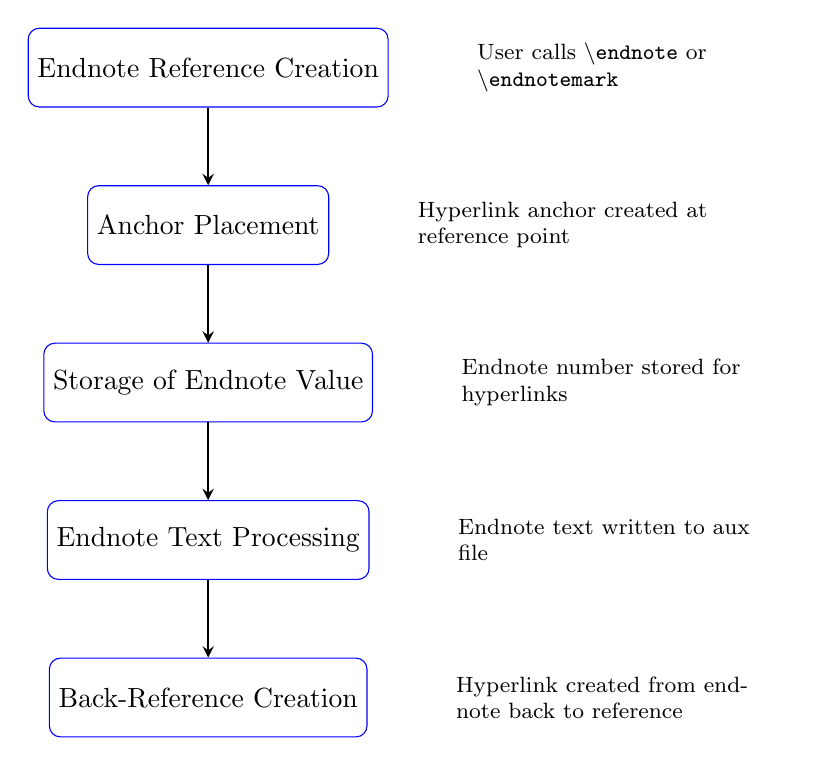
\begin{tikzpicture}[node distance=2cm]
  % Nodes
  \node (step1) [process] {Endnote Reference Creation};
  \node (step2) [process, below of=step1] {Anchor Placement};
  \node (step3) [process, below of=step2] {Storage of Endnote Value};
  \node (step4) [process, below of=step3] {Endnote Text Processing};
  \node (step5) [process, below of=step4] {Back-Reference Creation};
  
  % Arrows
  \draw [arrow] (step1) -- (step2);
  \draw [arrow] (step2) -- (step3);
  \draw [arrow] (step3) -- (step4);
  \draw [arrow] (step4) -- (step5);
  
  % Annotations
  \node [annotation, right=1cm of step1] {User calls \cmd{endnote} or \cmd{endnotemark}};
  \node [annotation, right=1cm of step2] {Hyperlink anchor created at reference point};
  \node [annotation, right=1cm of step3] {Endnote number stored for hyperlinks};
  \node [annotation, right=1cm of step4] {Endnote text written to aux file};
  \node [annotation, right=1cm of step5] {Hyperlink created from endnote back to reference};
\end{tikzpicture}
\caption{Hyperlink Creation Process}
\end{figure}

\subsection{Auxiliary Files Handling}

The package writes endnote content to an auxiliary file (\file{.ent}) that is later read when \cmd{theendnotes} is called. For each endnote, it stores:

\begin{enumerate}
  \item The formatted endnote number (for display)
  \item The raw endnote counter value (for hyperlinks)
  \item The endnote content
\end{enumerate}

\begin{tcolorbox}[colback=gray!5, colframe=gray!75, title=Sample .ent File Content]
\begin{verbatim}
\@doanenote{1}{1}
macro:->\protect \uppercase {T}his is the content of the endnote.
\@endanenote
\@doanenote{2}{2}
macro:->Second endnote with a \protect \url {https://example.com} link.
\@endanenote
\end{verbatim}
\end{tcolorbox}

\subsection{Hyperref Integration}

The package carefully integrates with \pkg{hyperref} by:

\begin{itemize}
  \item Creating anchor points using \cmd{hyper@@anchor}
  \item Creating hyperlinks using \cmd{hyper@linkstart} and \cmd{hyper@linkend}
  \item Preserving \cmd{href} and \cmd{url} functionality within endnotes
  \item Using a consistent naming scheme for hyperlink targets
\end{itemize}

\subsection{Technical Challenges and Solutions}

\begin{table}[h]
\centering
\begin{tabular}{p{4cm} p{10cm}}
\toprule
\textbf{Challenge} & \textbf{Solution} \\
\midrule
Preserving hyperlinks within endnotes & Save and restore \cmd{href} and \cmd{url} commands \\
Making endnote numbers work as hyperlinks & Store the raw endnote counter value alongside the formatted display value \\
Ensuring consistent rendering & Carefully redefine internal commands without breaking core functionality \\
Handling special characters in endnotes & Save category codes and restore them appropriately \\
Providing toggle functionality & Use \cmd{ifenotelinks} boolean toggle with conditional code execution \\
\bottomrule
\end{tabular}
\caption{Technical Challenges and Solutions}
\end{table}

\section{Advanced Examples}

\subsection{Basic Example with Bidirectional Links}

\begin{tcolorbox}[colback=gray!5, colframe=gray!75, title=Basic Example]
\begin{lstlisting}
\documentclass{article}
\usepackage{endnotes}
\usepackage{hyperref}
\usepackage{hyperendnotes}

\begin{document}

This is a paragraph with an endnote.\endnote{This is the content of the first endnote. It contains some explanatory text.}

Here is another paragraph with a second endnote.\endnote{This is the 
second endnote with a \url{https://example.com} hyperlink inside it.}

% Multiple references to the same endnote
This references the first endnote again.\endnotemark[1]

% Just a mark without text
Here is a mark without text.\endnotemark

% Just text without a mark
\endnotetext{This endnote has no mark in the text.}

\newpage
\theendnotes

\end{document}
\end{lstlisting}
\end{tcolorbox}

\subsection{Toggling Links On/Off}

\begin{tcolorbox}[colback=gray!5, colframe=gray!75, title=Toggling Links Example]
\begin{lstlisting}
\documentclass{article}
\usepackage{endnotes}
\usepackage{hyperref}
\usepackage{hyperendnotes}

\begin{document}

% Links enabled (default)
This endnote has links enabled.\endnote{This endnote has bidirectional hyperlinks.}

% Disable links
\enotelinksfalse
This endnote has links disabled.\endnote{This endnote does not have hyperlinks.}

% Re-enable links
\enotelinkstrue
This endnote has links enabled again.\endnote{This endnote has bidirectional hyperlinks.}

\newpage
\theendnotes

\end{document}
\end{lstlisting}
\end{tcolorbox}

\subsection{Customized Endnote Appearance}

\begin{tcolorbox}[colback=gray!5, colframe=gray!75, title=Customized Appearance Example]
\begin{lstlisting}
\documentclass{article}
\usepackage{endnotes}
\usepackage{hyperref}
\usepackage{xcolor}
\usepackage{hyperendnotes}

\begin{document}

% Customize endnote marks in text
\renewcommand{\makeenmark}{%
  {\color{blue}[\textsuperscript{\theendnote}]}%
}

% Customize endnote appearance in endnotes section
\makeatletter
\renewcommand*\@makeenmark{%
  \hbox{\color{blue}\textbf{\@theenmark.}}%
}

% Customize endnotes heading
\renewcommand{\enoteheading}{\section*{\color{blue}Notes \& References}}

% Add more space between endnotes
\renewcommand{\theendnotes}{%
  \immediate\closeout\@enotes
  \global\@enotesopenfalse
  \begingroup
  \makeatletter
  % ... [keep original code] ...
  \def\@doanenote##1##2##3>{%
    \def\@theenmark{##1}%
    \def\@theenvalue{##2}%
    \par\vspace{1em} % Increased spacing between endnotes
    % ... [keep rest of original code] ...
  }
  % ... [keep original code] ...
  \enoteheading
  \enotesize
  \input{\jobname.ent}%
  \endgroup
}
\makeatother

Sample text with customized endnotes.\endnote{This is a customized endnote.}
Another example.\endnote{Another customized endnote with \url{https://example.org}.}

\newpage
\theendnotes

\end{document}
\end{lstlisting}
\end{tcolorbox}

\section{Compatibility Considerations}

\subsection{Package Compatibility}

The \pkg{hyperendnotes} package is designed to work with specific versions of its dependencies:

\begin{itemize}
  \item \pkg{endnotes} package: Compatible with versions that follow the standard implementation pattern
  \item \pkg{hyperref} package: Compatible with most versions, but may require adjustments for very old or very recent versions
\end{itemize}

\subsection{LaTeX Engine Compatibility}

The package has been tested with:

\begin{itemize}
  \item pdfLaTeX
  \item XeLaTeX
  \item LuaLaTeX
\end{itemize}

\subsection{Known Issues}

\begin{enumerate}
  \item If the \pkg{endnotes} package is updated with changes to its internal commands, \pkg{hyperendnotes} may need updates to remain compatible.
  \item When using complex document classes or packages that redefine basic LaTeX commands, some conflicts may arise.
  \item Multiple compilation runs may be required for hyperlinks to work correctly, especially when endnotes are added or removed.
\end{enumerate}

\subsection{Conflict Resolution}

If conflicts occur with other packages:

\begin{itemize}
  \item Load \pkg{hyperendnotes} after potentially conflicting packages
  \item Check the loading order of packages, especially those that modify core LaTeX commands
  \item If needed, use \cmd{makeatletter} and \cmd{makeatother} to redefine specific commands after all packages are loaded
\end{itemize}

\section{Technical Reference}

\subsection{Internal Commands}

\begin{table}[h]
\centering
\begin{tabular}{>{\ttfamily}l p{8cm}}
\toprule
\textbf{Command} & \textbf{Purpose} \\
\midrule
\normalfont\cmd{@theenmark} & Holds the formatted endnote number \\
\normalfont\cmd{@theenvalue} & Holds the raw endnote counter value \\
\normalfont\cmd{@endnotemark} & Formats and places the endnote mark \\
\normalfont\cmd{@endnotetext} & Processes and writes endnote text \\
\normalfont\cmd{@doanenote} & Formats an individual endnote in the endnotes section \\
\normalfont\cmd{@endanenote} & Closes an individual endnote in the endnotes section \\
\bottomrule
\end{tabular}
\caption{Internal Commands}
\end{table}

\subsection{Hyperlink Naming Convention}

The package uses a consistent naming convention for hyperlink targets:

\begin{itemize}
  \item \texttt{Hendnotepage.\textit{n}} -- Target at the endnote mark in the text
  \item \texttt{Hendnote.\textit{n}} -- Target at the endnote in the endnotes section
\end{itemize}

Where \textit{n} is the endnote number.

\subsection{Modifying the Package}

For advanced users who need to modify the package:

\begin{tcolorbox}[colback=gray!5, colframe=gray!75, title=Modifying the Package]
\begin{lstlisting}
% Create a local copy of hyperendnotes.sty
% Make your changes to the local copy
% Load your custom version instead of the standard one:

\makeatletter
% Your modifications to commands here
\makeatother
\end{lstlisting}
\end{tcolorbox}

\section{Demonstration}

This section demonstrates the functionality of the \pkg{hyperendnotes} package in this document itself.

Here is a sample endnote with a hyperlink\endnote{This is a demonstration endnote. It includes a hyperlink to \url{https://www.latex-project.org/}.}. You can click on the endnote number to jump to the endnote, and then click on the endnote number in the endnotes section to jump back to this reference point.

Here's another endnote with different content\endnote{This second demonstration endnote shows how multiple endnotes are formatted and linked.}.

Notice how clicking on these endnote references takes you to the corresponding endnote at the end of the document, and clicking on the endnote numbers at the end brings you back to these reference points.

\subsection{Complex Example}

Here is a more complex example with multiple references and nested content:

First reference\endnote{This endnote contains a citation\cite{knuth1984texbook} and a nested URL \url{https://www.ctan.org/}.}.

Second reference\endnote{This endnote contains mathematical content: $E = mc^2$ and code: \texttt{function example() \{ return true; \}}}.

Third reference\endnote{This endnote contains a list:
\begin{itemize}
  \item First item
  \item Second item
  \item Third item with \url{https://example.com}
\end{itemize}
}.

\section{Conclusion}

The \pkg{hyperendnotes} package extends the functionality of the standard \pkg{endnotes} package by adding comprehensive hyperlink capabilities. It creates a more interactive document experience by enabling bidirectional navigation between endnote references and the actual endnotes.

Key benefits of the package include:

\begin{itemize}
  \item Enhanced navigation between text and endnotes
  \item Preservation of hyperlinks within endnote content
  \item Customizable appearance and behavior
  \item Toggle mechanism to enable/disable hyperlinks
  \item Compatibility with standard LaTeX workflows
\end{itemize}

The package is particularly valuable for long academic documents, technical manuals, and any publication where endnotes are used extensively.

\begin{thebibliography}{9}
\bibitem{knuth1984texbook} Knuth, D. E. (1984). The TeXbook. Addison-Wesley.
\end{thebibliography}

\vspace{2cm}
\theendnotes

\end{document}